%File: formatting-instruction.tex
\documentclass{sig-alternate}
%\documentclass[letterpaper]{article}

%\documentclass{aamas2013}
\usepackage{epstopdf}
\usepackage{amsfonts}
\usepackage{amsmath}
\usepackage{algorithmicx}
\usepackage{algpseudocode}
\usepackage{algorithm}
\usepackage{subcaption}
\usepackage{array}
%\fontsize{24}{6}
%\selectfont

%\usepackage{draftwatermark}
%\SetWatermarkScale{1}
%\SetWatermarkLightness{.9}
%\SetWatermarkAngle{-45}
%\SetWatermarkText{DRAFT DRAFT DRAFT DRAFT}


%\usepackage[usenames]{color}
\DeclareMathOperator*{\argmin}{argmin}

%\makeatletter
%\let\@copyrightspace\relax
%\makeatother

% if you are using PDF LaTex and you cannot find a way for producing
% letter, the following explicit settings may help

%\pdfpagewidth=8.5truein
%\pdfpageheight=11truein

\newfont{\mycrnotice}{ptmr8t at 7pt}
\newfont{\myconfname}{ptmri8t at 7pt}
\let\crnotice\mycrnotice%
\let\confname\myconfname%

\permission{Permission to make digital or hard copies of all or part of this work for personal or classroom use is granted without fee provided that copies are not made or distributed for profit or commercial advantage and that copies bear this notice and the full citation on the first page. Copyrights for components of this work owned by others than ACM must be honored. Abstracting with credit is permitted. To copy otherwise, or republish, to post on servers or to redistribute to lists, requires prior specific permission and/or a fee. Request permissions from permissions@acm.org.}
\conferenceinfo{GECCO'14,}{July 12--16, Vancouver, BC, Canada.}
\copyrightetc{Copyright 2014 ACM \the\acmcopyr}
\crdata{978-1-4503-2662-9/14/07\ ...\$15.00.\\
http://dx.doi.org/10.1145/2576768.2598385}

\clubpenalty=10000 
\widowpenalty = 10000

\begin{document}
    
%\AuthorsForCitationInfo{William Curran, Adrian Agogino, Kagan Tumer}

%\TitleForCitationInfo{Hierarchical Simulation for Complex Domains : Air Traffic Flow Management}

\title{Hierarchical Simulation for Complex Domains : Air Traffic Flow Management}

%\titlenote{For use with aamas2011.cls}}

% AUTHORS

\numberofauthors{3}

\author{
\alignauthor
William Curran\\
       \affaddr{Oregon State University}\\
       \affaddr{Corvallis, Oregon}\\
       \affaddr{curranw@onid.orst.edu}
\alignauthor
Adrian Agogino\\
       \affaddr{NASA AMES Research Center}\\
       \affaddr{Moffet Field, California}\\
       \affaddr{adrian.k.agogino@nasa.gov}
\alignauthor 
Kagan Tumer\\
       \affaddr{Oregon State University}\\
       \affaddr{Corvallis, Oregon}\\
       \affaddr{kagan.tumer@oregonstate.edu}
}
\maketitle


\begin{abstract}

A key element in the continuing growth of air traffic is the increased use of automation. The Next Generation (Next-Gen) Air Traffic System will include automated decision support systems and satellite navigation that will let pilots know the precise locations of other aircraft around them. This Next-Gen suggestion system can assist pilots in making good decisions when they have to direct the aircraft themselves. However, effective automation is critical in achieving the capacity and safety goals of the Next-Gen Air Traffic System. In this paper we show that evolutionary algorithms can be used to achieve this effective automation.

However, it is not feasible to use a standard evolutionary algorithm learning approach in such a detailed simulation. Therefore, we apply a hierarchical simulation approach to an air traffic congestion problem where agents must reach a destination while avoiding separation violations. Due to the dynamic nature of this problem, agents need to learn fast. Therefore, we apply low fidelity simulation for agents learning their destination, and a high fidelity simulation employing the Next-Gen technology for learning separation assurance. The hierarchical simulation approach increases convergence rate, leads to a better performing solution, and lowers computational complexity by up to 50 times.


%In dynamic multiagent learning it is common to execute thousands of trials before a well-performing policy is found. In complex domains, high fidelity simulations are typically needed to accurately depict the environmental impact of an agent action. Performing these trials can easily become computationally intractable. Alternatively, low fidelity simulations are computationally cheap, but are not detailed enough for many learning domains. In this work we develop a new technique that intelligently combines high fidelity and low fidelity simulation, allowing fast and accurate simulation to guide the multiagent evolutionary learning. We call this the hierarchical simulation approach. 

%However, leveraging satellite navigation greatly increases the complexity of the evolutionary learning problem. Additionally, in dynamic multiagent learning it is common to execute thousands of trials before a well-performing policy is found. In complex domains, high fidelity simulations are typically needed to accurately depict the environmental impact of an agent action. Performing these trials can easily become computationally intractable. Alternatively, low fidelity simulations are computationally cheap, but are not detailed enough for many learning domains. In this work we develop a new technique that intelligently combines high fidelity and low fidelity simulation, allowing fast and accurate simulation to guide the multiagent evolutionary learning. We call this the hierarchical simulation approach.

%We apply the hierarchical simulation approach to an air traffic congestion problem where agents must reach a destination while avoiding separation violations. Due to the dynamic nature of this problem, agents need to learn fast. Therefore, we apply low fidelity simulation for agents learning their destination, and a high fidelity simulation employing the Next-Gen technology for learning separation assurance. The hierarchical simulation approach increases convergence rate, leads to a better performing solution, and lowers computational complexity by up to 50 times.
\end{abstract}


\category{I.2.11}{Distributed Artificial Intelligence}{Intelligent Agents}
\terms{
Algorithms, 
%Management, 
%Measurement, 
%Documentation, 
Performance, 
%Design, 
%Economics, 
%Reliability%, 
Experimentation%, 
%Security, 
%Human Factors, 
%Standardization, 
%Languages, 
%Theory, 
%Legal Aspects, 
%Verification.
}
\keywords{Aerospace Industry, Simulation Optimization, Multi-agent Systems, Co-evolution}

\vspace{5mm}
\section{Introduction}

Automation is becoming an important aspect of air traffic control. Decision support systems, computer-based information acquisition, trajectory planning systems, and advisory systems are considered to be automation components related to Next Generation (Next-Gen) airspace \cite{next-gen}. With the addition of these systems, learning becomes computationally intractable and approximations need to be made, but with more approximations the learned policy becomes less representative of the real application. To resolve this issue, we develop an approach that use both high and low fidelity simulations. The high fidelity simulations include complex computation and are used during separation assurance, while the low fidelity simulation solves high level problems and are used for reaching a destination. Both fidelities are needed to fully understand the system.

Typical methods to alleviate computational complexity in complex systems have been applied during learning, one such example is transfer learning \cite{Pan:2010:STL:1850483.1850545}. Transfer learning has been shown to alleviate computational complexity by learning in a simple domain, and transferring that knowledge to a more complex domain. In transfer learning there are three key research questions: What to transfer, how to transfer and when to transfer. Each of these questions are difficult to answer and all are completely domain dependent. When the source domain and the target domain are loosely or not related, straight forward transfer learning does not work, and can lead to worse performance \cite{Pan:2010:STL:1850483.1850545}. Lastly, transfer learning requires a computable mapping from the source domain to the target domain, which isn't always easily achieved.

Other methods have been applied to the simulation as a whole \cite{eps23053}. An approximation of a high fidelity simulator can greatly speed up computation time, but subtle, yet important, details can be approximated or removed from the system. In complex domains, these important details are needed, but are no longer available or are approximated, adding error into the system. Over time this error can propagate throughout the system, invalidating results and leading to suboptimal learning. An example of this is air traffic simulation. Two popular approaches to simulating air traffic in the United States had been to develop Lagrangian models of each aircraft's dynamics, or to create aggregate models of the National Airspace (NAS) \cite{Bertsimas:1998:ATF:767667.768027, McNally, Mueller_analysisof}. When the aircraft's dynamics are taken into account, the simulation is accurate, but also time-intensive and complex. On the other hand, aggregate models can be used as an approximation of the Lagrangian models. When using only a low fidelity simulation, a lot of pertinent information is lost, but when using using a high fidelity simulator, such as the Lagrangian model simulations, the simulation cost becomes high.

Coordinating aircraft is also a critical and difficult task.  Cooperative Coevolutionary Algorithms (CCEAs) are well suited for evolving multiple populations simultaniously and evaluating fitness based on an individuals interactions with other agents in the system. Additionally, CCEAs are well suited for multiagent domains where robustness is a desirable quality, and agents need to succeed or fail as a team \cite{Panait:2005:CML:1090749.1090753}. The population member assignment generates a robustness well suited for the Next-Gen system, as a solution needs to be able to withstand sudden changes that are frequent in air traffic. Although robustness is nice, the key advantage of this multiagent approach is each agent only has to search a subspace of the entire state space.

%There are also many situations where approximation is simply not an option. For example, a 3rd party simulator cannot be modified or simplified, and the computational complexity associated with it must be reduced through other means. Using a hierarchical simulation becomes an ideal solution. 

Our motivation for this work borrows from the field of Economics. Macroeconomics studies the impact of national economic policies on growth, inflation and unemployment, where microeconomics studies the behavior of individual households and businesses. Microeconomics exists because macroeconomics cannot adequately explain the decision making of an individual, and macroeconomics exists because analyzing an individual cannot explain large scale effects on the economy. The same is true for low fidelity and high fidelity simulators. The low fidelity simulation is on a macro scale. It is a useful tool when analyzing the performance of many agents as a whole, but it does not detail an individual. On the other hand, high fidelity simulation is on a micro scale, and is a very useful tool when learning requires fine grained detail of an individual agent. They are both required in order to fully understand the system, and if one is used to attempt to understand the environment as a whole, useful information can be lost.


%Agents developed policies using traditional cooperative coevolutionary algorithms (CCEAs) evolving weights for neural networks. In CCEAs, each population member of an agent is randomly assigned with population members of other agents to create a team. Fitnesses assigned to population members are based on the interactions within a given team.  This team is evaluated and each population member is given a fitness. Once all population members have been assigned to a team, evolutionary subsampling is performed. For this evolutionary algorithm, we use 50 population members per agent for 2000 generations. 

%CCEAs are well suited for multiagent domains where robustness is a desirable quality, and agents need to succeed or fail as a team. The random population member assignment generates a robustness well suited for our domain, as a solution needs to be able to withstand sudden changes that are frequent in air traffic. Although robustness is nice, the key advantage of this multiagent approach is each agent only has to search a subspace of the entire state space. 

%Evolutionary algorithms are well suited for multiagent domains where robustness is a desirable quality, and agents need to succeed, or fail, as a team. The population member assignment generates a robustness well suited for the Next-Gen system, as a solution needs to be able to withstand sudden changes that are frequent in air traffic.

In this work we apply our hierarchical simulation evolutionary approach to an air traffic control congestion domain. In our domain agents must reach their destination quickly while simultaneously avoiding separation violations. A low fidelity simulator is used for reaching the destination quickly, while the high fidelity simulation takes advantage of the advanced Next-Gen \cite{next-gen} technologies, namely Automatic Dependent Surveillance-Broadcast (ADS-B). ADS-B is a satellite-based technology that provides aircraft information of other aircraft, such as position and velocity, and can be used to avoid separation violations. We find that combining a low fidelity and high fidelity simulator leads to faster convergence rate and faster computation time.

The remainder of this paper is organized as follows. Section 2 describes the related work in hierarchical methods, multiagent coordination and fitness function shaping, and prior work in air traffic control. In Section 3 we describe the domain we use, and in Section 4 we explain our approach in detail by developing a low fidelity simulator and high fidelity simulator and combine the two. Experimental results are then provided in Section 5, followed by the conclusion in Section 6.

\section{Background}

To motivate our approach, we introduce previous work performed in the field of agent-based simulation techniques and hierarchical methods, describe the fitness function shaping technique used in this work, and include a description and overview of the air traffic problem.

\subsection{Simulation Techniques}

Many simulation techniques leverage the concept of simultaneous use of multiple fidelity models. In general, they partition the environment and run a different model in each partition. Anh et al. \cite{Anh:2011:HMP:2183423.2183461} and Stylianou et al. \cite{Stylianou04scalablepedestrian} applied such a model toward pedestrian simulation. Anh et al. used low fidelity flow and distribution models to steer nonvisible agents along a network of nodes that describe the accessible areas of a city. They also use a high fidelity simulation to perform collision avoidance. Stylianou et al. applied a top-down approach where the movement of the pedestrians was computed using a low fidelity simulation, taking a global view of the model. This information is used for guiding a more detailed and realistic high fidelity simulation when the user zooms in to a specific region, thus maintaining the consistency. Both of these approaches focused on consistency and speed of the results, showing that a mixed fidelity simulation can be as accurate as a high fidelity simulation. Additionally, both works require a preprocessed environment and predefined transition functions between the agents models while switching fidelities.

%To remove the need for predefined transition functions, IVE:Virtual Humans' AI Prototyping Toolkit \cite{Brom:2007:SLD:1421879.1421881} and Java Environment for the Design of agent Interaction (JEDI) \cite{Kubera:2008:IAS:1567281.1567367} were introduced. IVE adapts the fidelity level of the agent according to the importance of the area in which the entity is located without having to tweak the model or change the agent's representation. In this way, IVE can be used to switch fidelities without the need for a transition function. JEDI accomplishes the same result by representing the environment as a large number of cells representing the high fidelity areas on the environment. Each cell contains a matrix of possible interactions, therefore transition functions are not needed to change fidelity levels. Both of these approaches require predefined knowledge of agent interactions, which is not easily found during learning.

An alternative to simultaneous fidelity models is to approximate the high fidelity simulation \cite{ Proper:2012:MDR:2343896.2344025,eps23053}. In the work by S{\'o}bester et al. they employ parallel updates by searching an expected improvement surface generated from a radial basis function model \cite{eps23053}. They find that this is an accurate approximation of the high fidelity model. Proper et al. on the other hand replaced a high fidelity air traffic simulation entirely with an event-based air traffic model \cite{Proper:2012:MDR:2343896.2344025}. In complex domains approximations introduce small errors, which over time can propagate throughout the system, deteriorating performance.
  
In this work, we employ the simultaneous use of multiple fidelity models in multiagent learning for coordination. In this problem, transition functions between the fidelity models cannot be found, the environment is generalized, and agent interactions cannot be predicted and must be learned.

\subsection{Hierarchical Learning}

Hierarchical methods decompose large problems into smaller ones, overcomes partial observability, and re-uses subtasks. This organizational structure leads to many benefits, such as faster learning and learning from fewer trials. MAXQ by Dietterich et al. \cite{Dietterich00hierarchicalreinforcement} decomposes a Markov Decision Process (MDP) into a hierarchy of smaller MDPs and decomposes the value function of the target MDP into an additive combination of the value functions of the smaller MDPs. Our work similarly decomposes a large task into many semi-independent smaller tasks, essentially simultaneously solving many smaller, and therefore easier problems.

Similar to hierarchical methods, task-based decomposition decomposes large problems into many smaller, more task-specific problems. Agents are grouped together in teams that are specialized for a specific task. An agent can explore more parts of the state relevant to its current task rather than exploring the entire state space, and therefore learn faster \cite{Doucette:2012:HTD:2330163.2330178, 4708962}. Task-based decomposition has been previously applied in robotics for cellular manufacturing \cite{399902}, where the complexity of the manufacturing process is too large for a straightforward multiagent approach.  Task-based decomposition has also been used in pattern recognition \cite{788664} to simplify image classification through the use of decomposing pattern classification problems based on the task required.

This work can be seen as a mixture of hierarchical methods and task-based decomposition. Task-based decomposition typically uses the same agent throughout learning, and hierarchical methods don't use different fidelity levels in their simulations. In this work, multiple agents control each aircraft and hand over control. Essentially this approach employs one agent per fidelity level per aircraft, meaning the lower fidelity simulations have agents that can learn much faster, receiving state information useful only to their specific task.

\subsection{Fitness Function Shaping}
Multiagent coordination is an important aspect of many domains, such as air traffic control \cite{tumer-agogino_jaamas12}, Robocup soccer \cite{AAMAS12-agmon} and power plant operations \cite{Colby:2012:SFF:2343576.2343637}. A learning or evolutionary algorithm will often convert a once computationally intractable search problem into a feasible guided search. 

In learning algorithms fitness function design is important in keeping convergence time low while keeping performance high. In many multiagent coordination domains there is a difference between maximizing the system-level fitness and maximizing a single agent's fitness. If an agent always takes the locally-optimal action, it does not always maximize the system-level fitness.

The difference evaluation function \cite{tumer-agogino_jaamas12} is evaluated such that each agent's fitness is related to the individual's contribution to team performance, therefore the signal-to-noise ratio is improved considerably. This leads to final better policies at an accelerated convergence rate, as well as overcoming the Tragedy of the Commons. The difference evaluation function is defined as:
%
\begin{equation} \label{eq:DifferenceReward}
D_i(z) = G(z) - G(z - z_i + c_i)\;,
\end{equation}

where \textit{z} is the system state, $z_i$ is the system state with agent $i$, and $c_i$ is a counterfactual replacing agent $i$. This counterfactual offsets the artificial impact of removing an agent from the system. For example, removing an aircraft from the system always artificially decreases the amount of congestion, which would provide a inaccurate fitness if a counterfactual is not used.

The difference evaluation function provides a compact encapsulation of the agent's impact on the system. It reduces the noise from other agents in the fitness function signal and has outperformed both system-level and local fitness functions in many congestion domains \cite{AAMAS12-agmon, tumer-agogino_jaamas12, Colby:2012:SFF:2343576.2343637}.

\subsection{Air Traffic Control}

The Next Generation (Next-Gen) Air Traffic System will replace the system in place by the FAA. For decades aircraft have been flying indirect routes over radar towers, causing increased delay and adding congestion to highly traveled intersections. Next-Gen is the upgrade to a satellite-based technology. Automatic Dependent Surveillance-Broadcast (ADS-B) navigation is part of this Next-Gen technology and will let pilots know the precise locations of nearby aircraft. However, pilots cannot directly comprehend all of the data for each nearby aircraft. Adding an evolutionary agent as a suggestion system for the pilot is an ideal way show the pilot only pertinent navigation information. This allows more aircraft in the sky while enhancing the safety of travel.

Two popular approaches to simulating the Air Traffic Flow Management Problem (ATFMP) had been to develop Lagrangian models of each aircraft's dynamics, and to create aggregate models of the NAS \cite{Bertsimas:1998:ATF:767667.768027, McNally, Mueller_analysisof}. In the Lagrangian model approaches, typically the trajectories of each aircraft are taken into account and either collision-avoidance or congestion-reduction is performed \cite{McNally}. This is an accurate and fine-grained approach to the ATFMP, but also time-intensive and complex. Aggregate models have been shown to simplify the NAS and therefore are a much simpler approach to the ATFMP. The aggregate models have been used in conjunction with linear programming to find solutions to air traffic flow \cite{Bertsimas:1998:ATF:767667.768027}, and linear algorithms to analyze departure, enroute and arrival delays \cite{Mueller_analysisof}.

In this work we chose to use a Lagrangian model of the NAS, receiving the benefits of a more detailed simulation. Each aircraft is simulated relative to their velocity, yaw, and pitch. 

\section{Domain}

This paper demonstrates the usefulness of the hierarchical simulation approach in an important air traffic congestion problem. Therefore, we discuss the aircraft traffic congestion problem first, and then show how to apply our approach with respect to that optimization problem. This section describes how we formulated a multiagent congestion problem by defining the scenarios and agents and developed an appropriate system evaluation function.

\subsection{Scenario}

We test our approach in two scenarios. In both scenarios, aircraft are lined up on the final approach to their destination. Each aircraft is 100 units above ground and 25 units from the aircraft arriving before and after themselves. Initial orientations of each aircraft are assigned to be toward the destination airport and initial starting locations begin at 125 units away from the destination airport. An amount of gaussian noise ($\sigma = 5$, $\mu = 0$) is then added to the starting location of each aircraft. Lastly, the speed of each aircraft is held statically at 1 unit.

In the first scenario, there are two airports, and a set of 6 aircraft arriving at each airport. In this scenario there is one intersection point where aircraft flying a direct route trajectory can reach potential separation violations. The goal in this scenario is to show our approach adequately optimizes the delay to the aircraft's destination while incurring no separation violations.

In the second scenario there are 6 airports with 10 aircraft arriving at each airport. Again, the aircraft are lined up on a final approach vector. In this scenario each aircraft must go through three intersection points, with a total of 9 intersection points on the map. Our goal in this scenario is to see what issues occur in later intersections when an aircraft must switch many times between a low fidelity and high fidelity simulation. We also would like to see how our approach scales to larger systems.

We measure the performance in each scenario by computing the overall delay and congestion of all aircraft:
%
\begin{equation}
P(z) = \sum_{a \in A}{(\tau_{opt, a} - \tau_a) - C(z)}
\end{equation}

where $C(z)$ is the separation violation penalty (Equation \ref{eq:CongestionReward}), and $\tau_{opt, a}$ is the optimal time taken by aircraft $a$ to land as if it took a straight-line route from its starting location to its destination and $\tau_a$ is the actual time taken by aircraft $a$ to land. If an aircraft does not land, the negative of the total number of time steps is used, in this case $-600$. 
%\begin{figure}
%\centering
%\begin{subfigure}[b]{0.65\columnwidth}
%                \centering
%                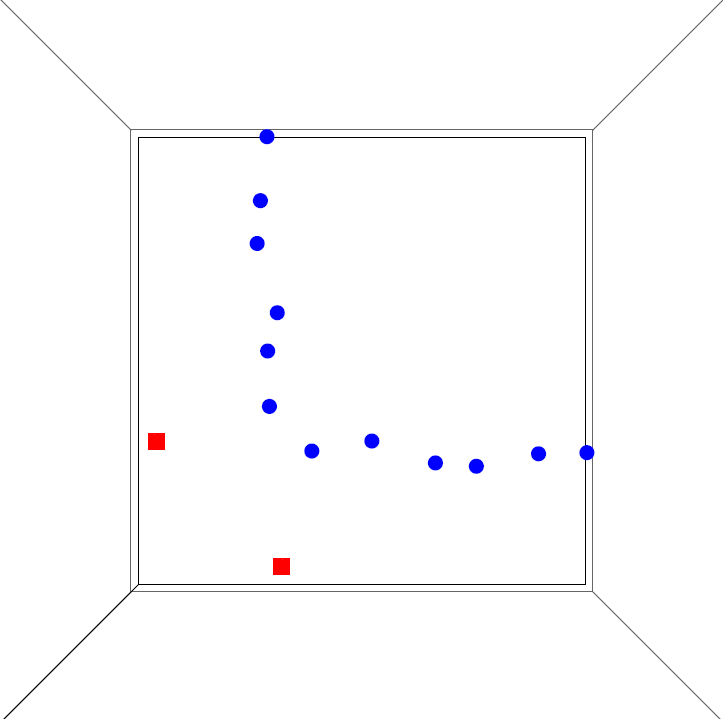
\includegraphics[width=1\columnwidth]{Animate3d-12}
%                \caption{12 aircraft}
%                \label{fig:12Aircraft}
%\end{subfigure}%
%\\
%\begin{subfigure}[b]{0.65\columnwidth}
%                \centering
%                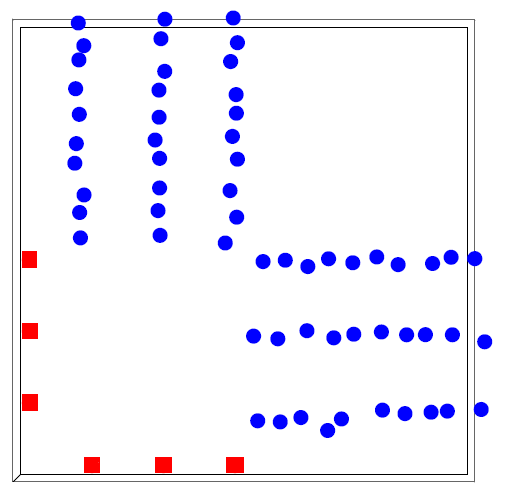
\includegraphics[width=1\columnwidth]{Animate3d-60}
%                \caption{60 aircraft}
%                \label{fig:60Aircraft}
%\end{subfigure}%
%\caption{(a). With the 12 aircraft scenario, we want to see if our approach adequately allows aircraft to reach their destination %quickly while allowing no separation violations. (b). With the 60 aircraft scenario we would like to see how our approach scales to %larger systems. Blue dots are aircraft and red squares are airports.}
%\label{fig:Scenarios}
%\end{figure}


\subsection{Agent Definition}
Agents actions are continuous and they may choose to change yaw by up to 1 radian in a positive or negative direction and change their pitch by up to 2 radians positively or negatively for one time step. Each aircraft's speed is held static, therefore the steeper it ascends or descends the slower it moves toward its destination. Agents dynamics are modeled according to the equations:
%
\begin{equation}
\begin{split}
&dx = |cos(pitch)| * cos(yaw) \\
&dy = |cos(pitch)| * sin(yaw) \\
&dz = sin(pitch) \\
\end{split}
\end{equation}

Each agent receives a state relative to their current simulation fidelity. Agents in the low fidelity simulations simply receive a state representing the aircraft relative to its destination, and agents in the high fidelity simulations receive a state that include the positions of nearby aircraft and the low fidelity state. This is explained in far more detail in Section 4. 

\subsection{Agent Policies}
Agents developed policies using traditional cooperative coevolutionary algorithms (CCEAs) evolving weights for neural networks. In CCEAs, each population member of an agent is randomly assigned with population members of other agents to create a team. Fitnesses assigned to population members are based on the interactions within a given team.  This team is evaluated and each population member is given a fitness. Once all population members have been assigned to a team, evolutionary subsampling is performed. For this evolutionary algorithm, we use 50 population members per agent for 2000 generations. 

%CCEAs are well suited for multiagent domains where robustness is a desirable quality, and agents need to succeed or fail as a team. The random population member assignment generates a robustness well suited for our domain, as a solution needs to be able to withstand sudden changes that are frequent in air traffic. Although robustness is nice, the key advantage of this multiagent approach is each agent only has to search a subspace of the entire state space. 


\subsection{Fitness Evaluation}
It is extremely important for pilots to keep a safe distance from other aircraft, therefore our goal in this work is to remove all separation violations, while simultaneously incentivizing aircraft to get to their destination in a timely manner. Therefore, the system-level fitness evaluation we developed focuses on the cumulative delay ($\delta$) and congestion ($C$) throughout the system:
%
\begin{equation}
G(z) = (\delta(z) + -C(z))\;,
\end{equation}

where $\delta(z)$ represents the delay in the system, and $C(z)$ is the total penalty for congestion violations.

The delay is defined by the sums of the difference between the straight-line distance to the goal during the last time step and the straight-line distance to the goal the current time step, such that the maximum value for each sum is the speed of aircraft $a$:
%
\begin{equation} \label{eq:DistanceReward}
\delta(z) = \displaystyle\sum\limits_{a \in A} \eta(a_{t-1},a_{dest}) - \eta(a_{t},a_{dest})\;,
\end{equation}

where $\eta(a_{t},a_{dest})$ is the distance from aircraft $a$ at time $t$ and aircraft $a$'s destination.

The total congestion penalty is the summation of violations per time step:
%
\begin{equation} \label{eq:CongestionReward}
C(z) = \displaystyle\sum\limits_{a_1 \in A} \displaystyle\sum\limits_{a_2 \in A} -\omega * \theta(\eta(a_1,a_2))\;,
\end{equation}

where $\theta(\eta(a_1,a_2))$ is a step function that is 1 if aircraft $a_1$ and $a_2$ are close enough to cause a violation, and 0 otherwise, and $\omega$ is the weight placed upon congestion, 1000 for our setup.

\section{Hierarchical Simulation}

The hierarchical simulation requires three main steps for agents to learn well-developed policies: formulating the low fidelity simulation, formulating the high fidelity simulation, and combining the two. This section will describe how to properly develop and combine these simulations with respect to the aircraft optimization problem.

\subsection{Low Fidelity Simulation}

Our low fidelity simulation includes very little detail of the environment, and is therefore very computationally inexpensive. Environment information for each agent includes only the location of its aircraft and the location of the aircraft's destination airport. Due to this minimal representation, agents in this simulation receives a simple state space and fitness function.

The agents in the low fidelity simulation are given a state that only includes the $\Delta heading$ to their destination, and the fitness function calculated as the change in distance to their destination (Equation \ref{eq:DistanceReward}). Since the low fidelity simulation includes all of the agents, many actions simultaneously impact the system environment, causing the fitness for a specific agent to become noisy with the actions of other agents. An agent would have difficulty evolving to an optimal solution using such a noisy fitness evaluation signal. A difference evaluation function reduces much of this noise (Equation \ref{eq:DifferenceReward}), and is easily derived from the system-level delay function (Equation \ref{eq:DistanceReward}):
%
\begin{equation} \label{eq:DistanceReward-Difference}
D_i(z) = \delta(z) - \delta(z - z_i + c_i)\;,
\end{equation}

where $\delta(z)$ is the delay fitness function with all agents and $\delta(z - z_i + c_i)$ is the delay fitness function with agents $i$ removed from the system and replaced with counterfactual agent $c_i$. This counterfactual represents the aircraft taking a locally optimal action toward it's destination. 

\subsection{High Fidelity Simulation}

Our high fidelity simulation takes advantage of the advanced Next-Gen \cite{next-gen} technologies, namely Automatic Dependent Surveillance-Broadcast (ADS-B). ADS-B is a satellite-based technology that provides aircraft information of other aircraft, such as position and velocity. 

ADS-B technology provides pilots information of other aircraft nearby, but pilots (and agents) cannot use all of this information, as the state space would become too large. For this reason, we model this limitation by only allowing agents to observe x, y and z locations of aircraft within 10 units.

Since the ADS-B technology is not currently implemented, different approaches of using ADS-B is a current area of research. Yildiz et al. \cite{Adrian-next-gen} modeled the pilot as being able to observe a limited section of the space in front of them, essentially discretizing the space in front of the agent into regions, and including 8 additional binary states, one for each region. This approach worked well in a 2D environment, but with a 3D environment the state space would need to be increased to at least 24 regions, 8 in front, 8 above and 8 below. 

Our ADS-B approach is simplified. It simply includes the relative x, y and z location of the nearest aircraft within its simulation. This approach involves a much smaller state representation than Yildiz et al. since it only includes the aircraft closest to the agent and the distance discretized into 10 bins. It also covers a larger area of the environment, which we predict will allow the agent to make more informed decisions.

The fitness function for the high fidelity simulation includes penalties for violations and incentives for arriving at the airport quickly:
%
\begin{equation} \label{eq:Global-HighFid}
G(z) = \delta(z) + -C(z)\;,
\end{equation}

where $C(z)$ is Equation \ref{eq:CongestionReward} and $\delta(z)$ is Equation \ref{eq:DistanceReward}.

We use the global evaluation function in the high fidelity simulations because only a few agents are using the high fidelity simulation at one time (This is explained further in the next section). Additionally, the difference evaluation function heavily biases the evolutionary search. If an agent takes an action that prevents a violation, that population member receives a very high fitness, and future mutations will search around that area of the state space. It was often during preliminary analysis that particular part of the state space had a high chance of being efficient at avoiding a violation in one particular orientation, but performed poorly at reaching its destination, or avoiding aircraft in other orientations, therefore we did not use the difference evaluation.

\subsection{Applying Hierarchical Simulation}
A key part of this research is how the high and low fidelity simulation interact. Each simulator contains its own set of agents, so when one simulator takes over, the aircraft that are switching fidelity levels are now being controlled by different agents. The differences between the low fidelity and high fidelity agents are the state inputs and fitness evaluation functions. These two sets of agents must learn to cooperate together in order for this approach to be viable. 

To switch from the low fidelity simulation to the high fidelity simulation, an aircraft needs to be within 10 units of another aircraft. At this point those two aircraft switch to a high fidelity agent and are ran in the same high fidelity simulation independently of other agents. If another aircraft enters within 10 units of one of these two aircraft, they are also added to the same high fidelity simulation as the original two. Independent simulations allowed us to calculate a global fitness relative to agents within that simulation (See Figure \ref{fig:60AircraftHF}). This greatly reduces the noise of other aircraft during learning.

Since the state for the low fidelity agents involves simply the angle from the aircraft to their destination, the agent has no knowledge of when the high fidelity agents are going to take over. During preliminary analysis of this approach, we discovered interesting emergent behavior when the high fidelity and low fidelity agents learned simultaneously. Since the high fidelity agents learned slower, due to a larger state space, they led the aircraft to a highly suboptimal location during early learning. Once the low fidelity simulation took over again, the aircraft was in an unexplored part of the state space, and the agent was required to learn how to lead the aircraft to its destination. Additionally, the low fidelity simulation can learn how to lead an agent to its destination much faster than the high fidelity simulation, due to the simpler state space. This ultimately led to the high fidelity simulation to have caused the low fidelity simulation to receive a worse fitness. 

Since the agents in the low fidelity simulation received a lower fitness due to the actions taken by the high fidelity simulator, the agents in the low fidelity simulation ``learned'' to avoid situations where the high fidelity simulation took over. Due to the high fidelity simulator only taking over the agent when a potential conflict is detected, the low fidelity agent indirectly began learning to avoid violations. Indirectly teaching agents on the simulation level is an interesting emergent behavior and is a topic in future work.

\begin{figure}
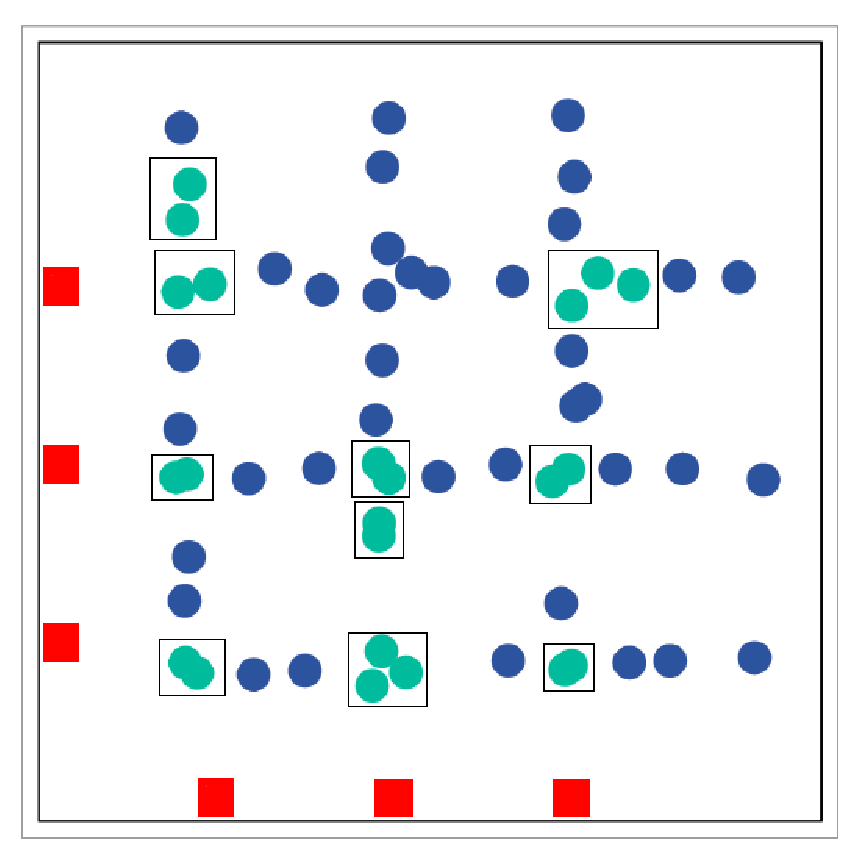
\includegraphics[width=.75\columnwidth]{Animate3d-60HF-FixedColor.eps}
\centering
\caption{Aircraft within boxes are in independent high fidelity simulations, aircraft not in boxes are in the same low fidelity simulation, and squares are airports. Note that the environment is in 3D, so agents look like they are within a separation violation, but are actually above or below each other. This situation is during the 60 aircraft scenario.}
\label{fig:60AircraftHF}
\end{figure}

Due to this emergent behavior, we do not train the high fidelity and low fidelity agents simultaneously. Instead, we borrow from the field of transfer learning. We first train a set of low fidelity agents to convergence in a large set of simple environments. We vary the starting location and orientation of each aircraft, and train the agent to reach its destination. Once trained, these agents are capable of always reaching their destination from any starting location and orientation. Low fidelity agents are held static, and used in our scenarios while we trained high fidelity agents in our scenarios.

Since agents were are active during every time step, their fitness functions need to be slightly modified. If agent $a$ is active for 400 time steps, and receives the same fitness as agent $b$, who was active for 300 time steps, agent $b$ performed better than agent $a$. We solve this problem by dividing each agent's fitness by their number of active time steps, assigning each agent their average fitness per time step. 

\section{Results}

In this section we test our simulation hierarchy approach in the air traffic domain and compare it to the performance of using a high fidelity only approach. We show general benefits of using a simulation hierarchy, including faster convergence and faster computation. Lastly, we show that due to the low fidelity and high fidelity separation, the simulation hierarchy approach is very robust to noise. All graphs in this section were computed using 10 statistical runs, and error bars are included.

\subsection{Performance}

The key benefit of using a simulator hierarchy is the increased speed of convergence. Agents in the low fidelity simulation are only concerned with reaching their destination. In this domain, this is a trivial problem to solve, and agents converge very fast to optimal. When adding in violation constraints, the problem becomes much harder. Agents are required to coordinate with each other to avoid separation violations. If only one fidelity simulator is being used, this problem becomes more difficult. Agents using only a high fidelity simulator will need to learn how to reach the destination while simultaneously learning to coordinate. If one agent evolves to a policy that allows an aircraft to reach the destination faster, but that policy leads to a separation violation, another agent must also have evolved to coordinate with that agent, all within the same simulation. This makes policies that perform separation coordination and reach their destination difficult to find. 

\begin{figure}
\centering
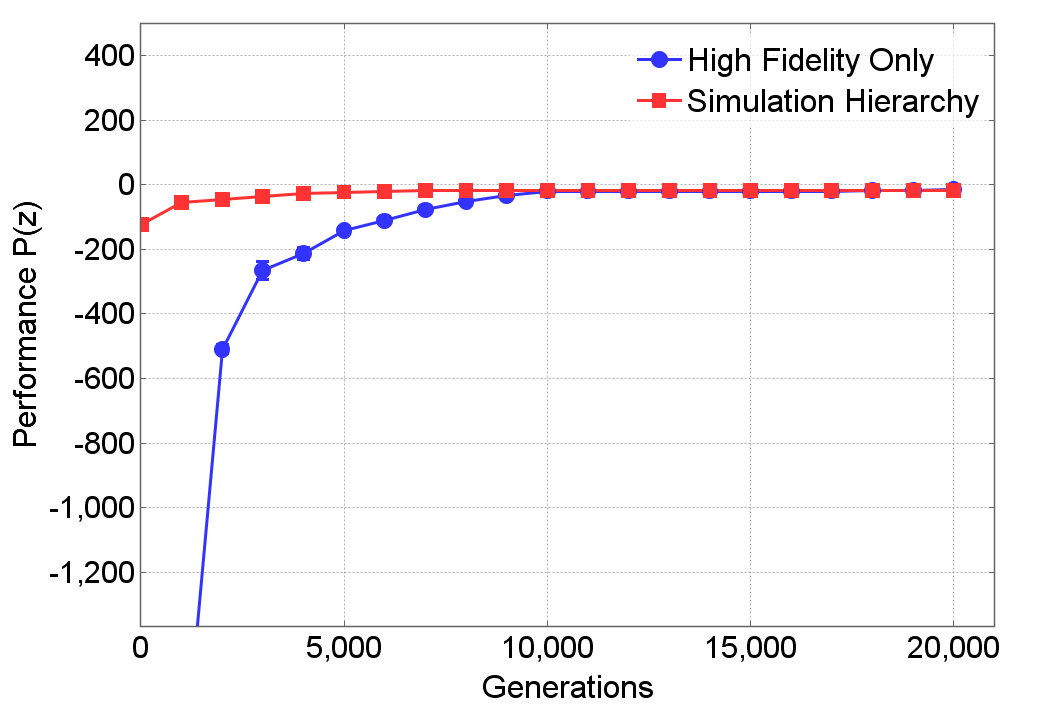
\includegraphics[width=.75\columnwidth]{SmallPerformance.eps}
\caption{The simulation hierarchy approach and high fidelity only approach converged to the same performance. However, the simulation hierarchy approach reached that level of performance much faster, and with less computation.}
\label{fig:12Performance}
\end{figure}


When using a simulation hierarchy, the agents in the low fidelity simulation can quickly learn how to reach their destination, while the high fidelity agents only turn on when a separation violation might occur. This means the high fidelity agents need only care about a very small portion of the state space, and will also learn much faster. This also means that we can easily perform transfer learning since the low fidelity aircraft are not coordinating. As long as the low fidelity agents can learn how to reach their destination from any location, which again is an easy problem to solve, they do not need to learn further. Only the high fidelity agents compute their fitness during each time step they are active.

As mentioned in Section 4.2, the difference evaluation function can't be used in the high fidelity simulation, and we have to use a global fitness evaluation function. The global evaluation function is easily computable, but does not perform well with many agents in a congestion domain \cite{AAMAS12-agmon, Colby:2012:SFF:2343576.2343637, tumer-agogino_jaamas12}. This isn't a problem when we use simulation hierarchies. Each group of agents within a high fidelity simulator are treated independently of each other, so the global fitness function represents only a few agents at a time. The global fitness function is a very good learning signal when only a few agents are included. When using only the high fidelity simulator, every agent receives the same global fitness function, and is therefore given a noisier global fitness function. 

This increased convergence rate makes it much easier to scale to larger systems, since well performing policies become much easier to find. As you can see from Figure \ref{fig:12Performance}, using a hierarchical simulation in the smaller scenario leads to a much faster convergence rate to an equally performing solution. In this scenario, we apply transfer learning in the low fidelity simulation, which gives it a much higher starting performance. This scenario is not complex enough for the simulation hierarchy approach to see any performance benefits over the high fidelity only approach. However, the high fidelity only approach takes much more computation to reach that same level of performance, as will be discussed in the next section.

In the higher complexity scenario, the simulation hierarchy approach is able to converge to a well performing solution very quickly (Figure \ref{fig:60Performance}). This is due to the high fidelity simulations being treated independently of each other, and the low fidelity transfer learning. The high fidelity only approach should theoretically eventually reach the performance of the simulation hierarchy, but at a huge cost of computation.

In these experiments, transfer learning was not used for the high fidelity only approach due to the noise in the global fitness function. In both approaches, once an agent transferred to a larger environment, it was able to reach its destination, but not without incurring violations. The global fitness function in the high fidelity only approach was too noisy for agents to learn to avoid these violations, and therefore have a much worse performance than if transfer learning was not used. In the hierarchical simulation approach, the fitness function is less noisy, and agents are able to quickly learn to avoid violations.

\begin{figure}
\centering
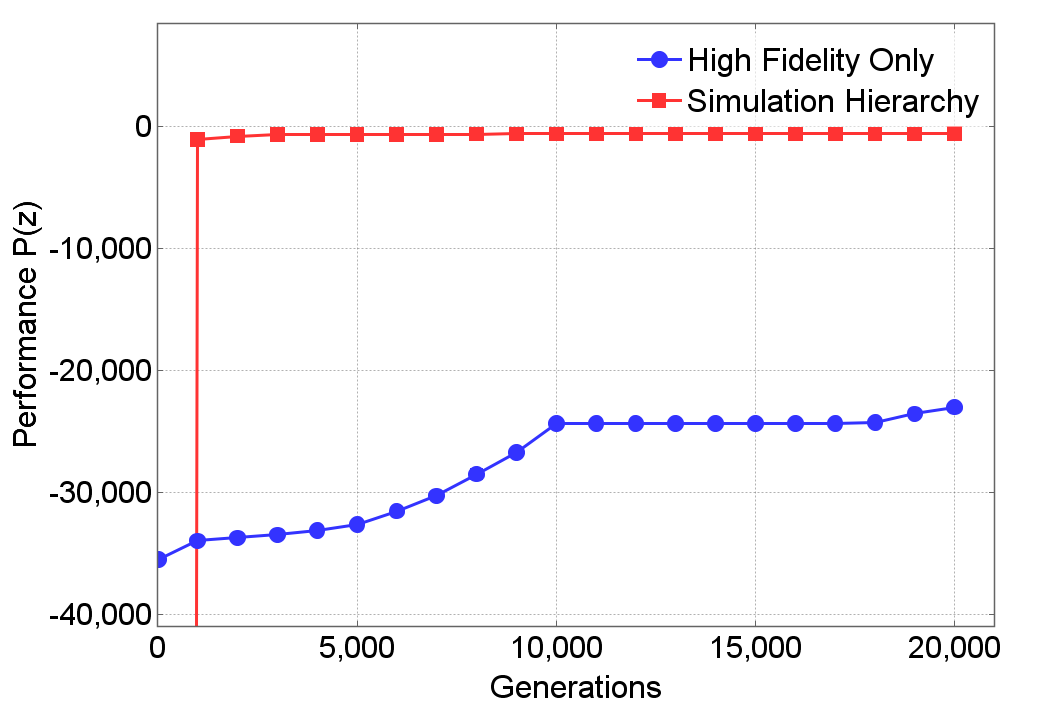
\includegraphics[width=.75\columnwidth]{LargePerformance.eps}
\caption{The simulation hierarchy approach outperformed the high fidelity only approach due to a less noisy fitness function and transfer learning. Since each high fidelity simulation is treated independently of each other, the global fitness function accurately encapsulates how each agent affects the environment.}
\label{fig:60Performance}
\end{figure}

\subsection{Speed}

Decreasing the computational complexity of a simulator is extremely useful in learning. When performing hundreds of thousands of trials, even a small speedup of one simulation step can impact overall computation time by magnitudes. In complex domains this decreased computation time leads to an ability to scale to larger systems, add more agents, or use more accurate physical models. 

When using only the high fidelity simulation, computing the high fidelity state requires each agent to compute a larger state: x, y and z of the closest aircraft, and the degree between the aircraft and the destination. In addition, due to the more complex state space and additional neural network inputs, a larger neural network is needed to fully learn the system, further increasing computation time. 

In a high fidelity simulator, it is common for systems to need to sacrifice speed to compute additional useful information, such as querying 3rd party software or performing additional computation. In this scenario, this additional information is through the use of the ADS-B system, which is used in the high fidelity simulator to compute the relative location of nearby aircraft. Note that the ADS-B system data received will be 1 MB, with a 50MB/s signal \cite{ads-b}. Therefore, we added an additional computational cost of 0.02 second when using the ADS-B technology to give a more realistic computational complexity analysis the high fidelity simulator.

When using the hierarchical simulation approach, agents are required to compute the full state a small number of time steps. Agents are in the low fidelity simulation unless a potential separation violation can occur. Table \ref{Table:Timing} shows the computation time per simulation step of the different scenarios. During learning we call the simulation 200,000 times, for 600 time steps each, therefore even a small speed up here leads to an extremely large time savings. 

When using the simulation hierarchy approach without penalties to the high fidelity simulation, the computation time required per simulation step was about half of when using the high fidelity only approach. This is due to the fast computational speed of the low fidelity simulation, and only switching to the slower, yet more detailed, high fidelity simulation to perform collision avoidance. When adding in the penalties for the ADS-B system, the simulation hierarchy approach was 13x faster per simulation step in the smaller scenario, and 52x faster in the larger scenario. This is one of the key benefits of using the simulation hierarchy approach. 

\begin{table}
\begin{tabular}{| c |c|c|c|c|c|}
\hline
 & \multicolumn{2}{ c|} {Simulation time (s)} &  &  \\

Scenario & No Penalty & Penalty & HF calls &  LF calls \\
\hline
12-HF+LF & 0.02 & 2.94 & 146 & 1702 \\
\hline
12-HF & 0.05 & 39.23 & 1959 & 0 \\
\hline
60-HF+LF & 0.1 & 11.68 & 579 & 21789\\
\hline
60-HF & 0.25 & 617.21 & 30848 & 0\\
\hline
\end{tabular}
\caption{The amount of computation time required per simulation step was much smaller when using the simulation hierarchy approach both with and without the penalty to the high fidelity simulation.}
\label{Table:Timing}
\end{table}

In an application that uses the difference evaluation function, the computational speed up would be even greater. The difference fitness function is a useful tool for accurately evaluating a policy, but it is often computationally expensive, especially when resimulation is required. This approach can speed up the difference fitness function computation in a high fidelity simulation, since the number of agents in each independent high fidelity simulation is very small. This can easily turn a once intractable problem into a tractable one.

\vspace{10mm}
\subsection{Accuracy}

One of the key concerns of using a simulator hierarchy is whether or not the simulation as a whole is accurate enough for the agents to learn a well performing policy. We argue that as long as the correct fidelity transition function is used, a simulation hierarchy is as accurate as simply using a high fidelity simulator, except with a much faster convergence rate and at less computational complexity. As shown in Figure \ref{fig:12Performance}, the high fidelity only approach eventually reaches the performance of simulation hierarchy approach, but at a much slower convergence rate. Additionally, as shown in Table \ref{Table:Timing}, the high fidelity only approach is much more computationally expensive. 

We further analyze the robustness of the simulator hierarchy approach by adding noise to the low fidelity simulation. There is an interesting cost-benefit study here. If the mechanism deciding which fidelity an agent uses is centralized, and therefore noiseless, adding noise to the low fidelity system state will hardly hurt performance. This is because if an agent is within the fidelity transition function criteria, the high fidelity simulation takes over and insures there will be no separation violations. This centralized approach is ideal, but comes with the typical problem of centralized approaches. If this decision mechanism has an error, or breaks down, all of the aircraft in the system will be at risk. 

If the fidelity transition function is included in the agent design, it becomes decentralized and doesn't suffer from a system wide break down if one mechanism incurs an error. However, since the fidelity transition function is on a per-agent basis and is included in the agent definition, it must include the noise that the agent receives. If the noise is greater than the fidelity transition function criteria, agents may be in a low fidelity simulation when they should be attempting to avoid a violation. The agent is in a low fidelity simulation and does not realize it is close to another agent. This issue does not occur if the noise is less than the fidelity transition function criteria, as the high fidelity simulation will take over before a violation can occur.

We simulate this by adding a static amount of noise modified by a normal distribution noise model to the low fidelity simulation:
%
\begin{equation}
\eta = N(0,1) \pm r
\end{equation} 

where $N(0,1)$ is a normal distribution with $\mu = 0$ and $\sigma = 1$, and $r$ is a static value representing a constant noise being added or removed from the Gaussian distribution.

Adding Gaussian noise to the x, y, and z locations during each time step introduced noise in both the state information and the fidelity transition function. As shown in Figure \ref{fig:NoiseAllRuns}, this noise introduction affects performance negatively, but this approach is still very robust to noise.

\begin{figure}
\centering
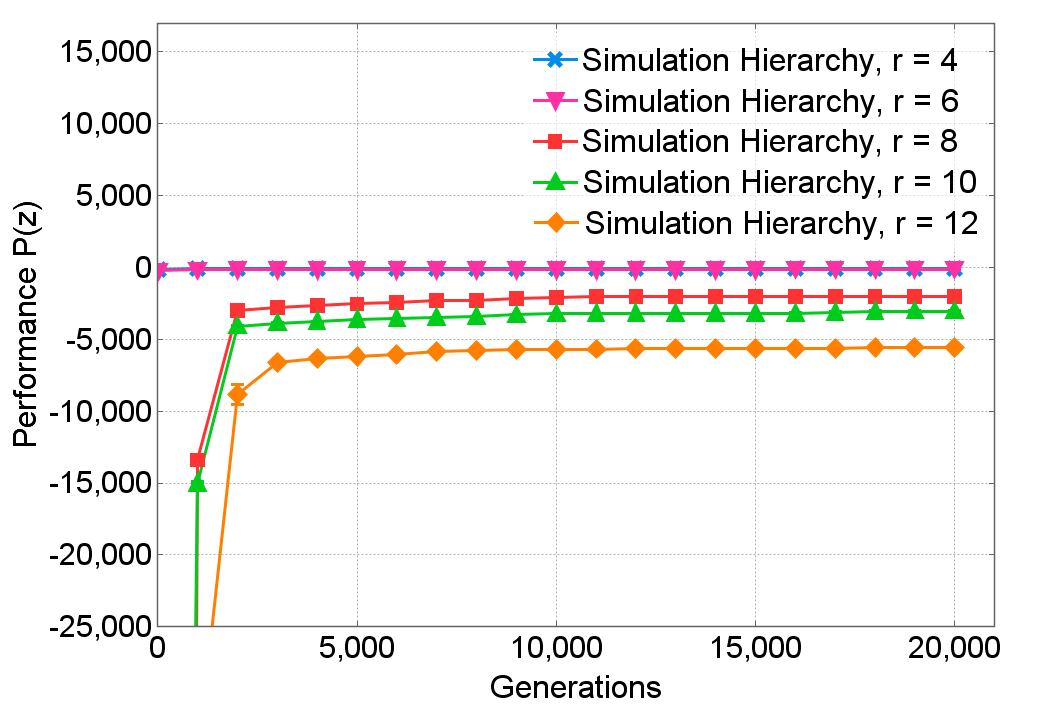
\includegraphics[width=.75\columnwidth]{NoiseNew.eps}
\caption{Adding/subtracting up to 6 units for noise while adding $N(0,1)$ Gaussian noise only slightly affected performance. Performance was largely affected when the total noise could potentially become greater than the fidelity transition function criteria. }
\label{fig:NoiseAllRuns}
\end{figure} 

\section{Conclusion}
This paper introduces the simulation hierarchy approach, an approach that uses both a high and low fidelity simulation and receives benefits from both. High fidelity simulation leads to higher quality learning due to a more detailed state space, but at a large cost of computation. On the other hand, low fidelity simulation has a less detailed state space, but is computationally inexpensive.

In this work, we show that the simulation hierarchy approach leads to a faster convergence rate while simultaneously reducing the computational complexity of running simulations. Learning using simulation hierarchies leads to a similar performing solution in the low complexity scenario at a 13x reduction in time complexity. In the higher complexity scenario, learning with simulation hierarchies leads to a much better performing solution at a 52x reduction in time complexity. When using simulation hierarchies, treating each high fidelity simulation as an independent simulation led to this increase of performance, while switching between the high and low fidelity simulation led to the decrease in computation time and robustness to noise, resulting in a fast, robust, and well performing approach.

\label{sec:CONCLUSION}


\bibliographystyle{plain}
\bibliography{thesis}

\end{document}
